%! Author = Len Washington III
%! Date = 8/25/2023

% Preamble
\documentclass[12pt]{report}

% Packages
\usepackage{titling}
\title{Aug 25, 2023 Notes}
\usepackage{math252notes}

% Document
\begin{document}

\setcounter{chapter}{1}
\chapter{First-Order Differential Equations}
%<*Section-2.1>
\section{Solution Curves Without a Solution}\label{sec:solution-curves-without-a-solution}
Given a 1st order D.E. $y'=f(x,y)$, $y'$ is the slope of the tangent line at any point $(x_{0},y_{0})$ on a solution curve

\example
\[y'=f(x,y)=x+y\]
\begin{itemize}
	\item $f(0,0)$=0
	\item $f(1,0)$=1
\end{itemize}

\subsection{Slope/Direction Fields}\label{subsec:direction-fields}
\begin{figure}[H]
	\centering
	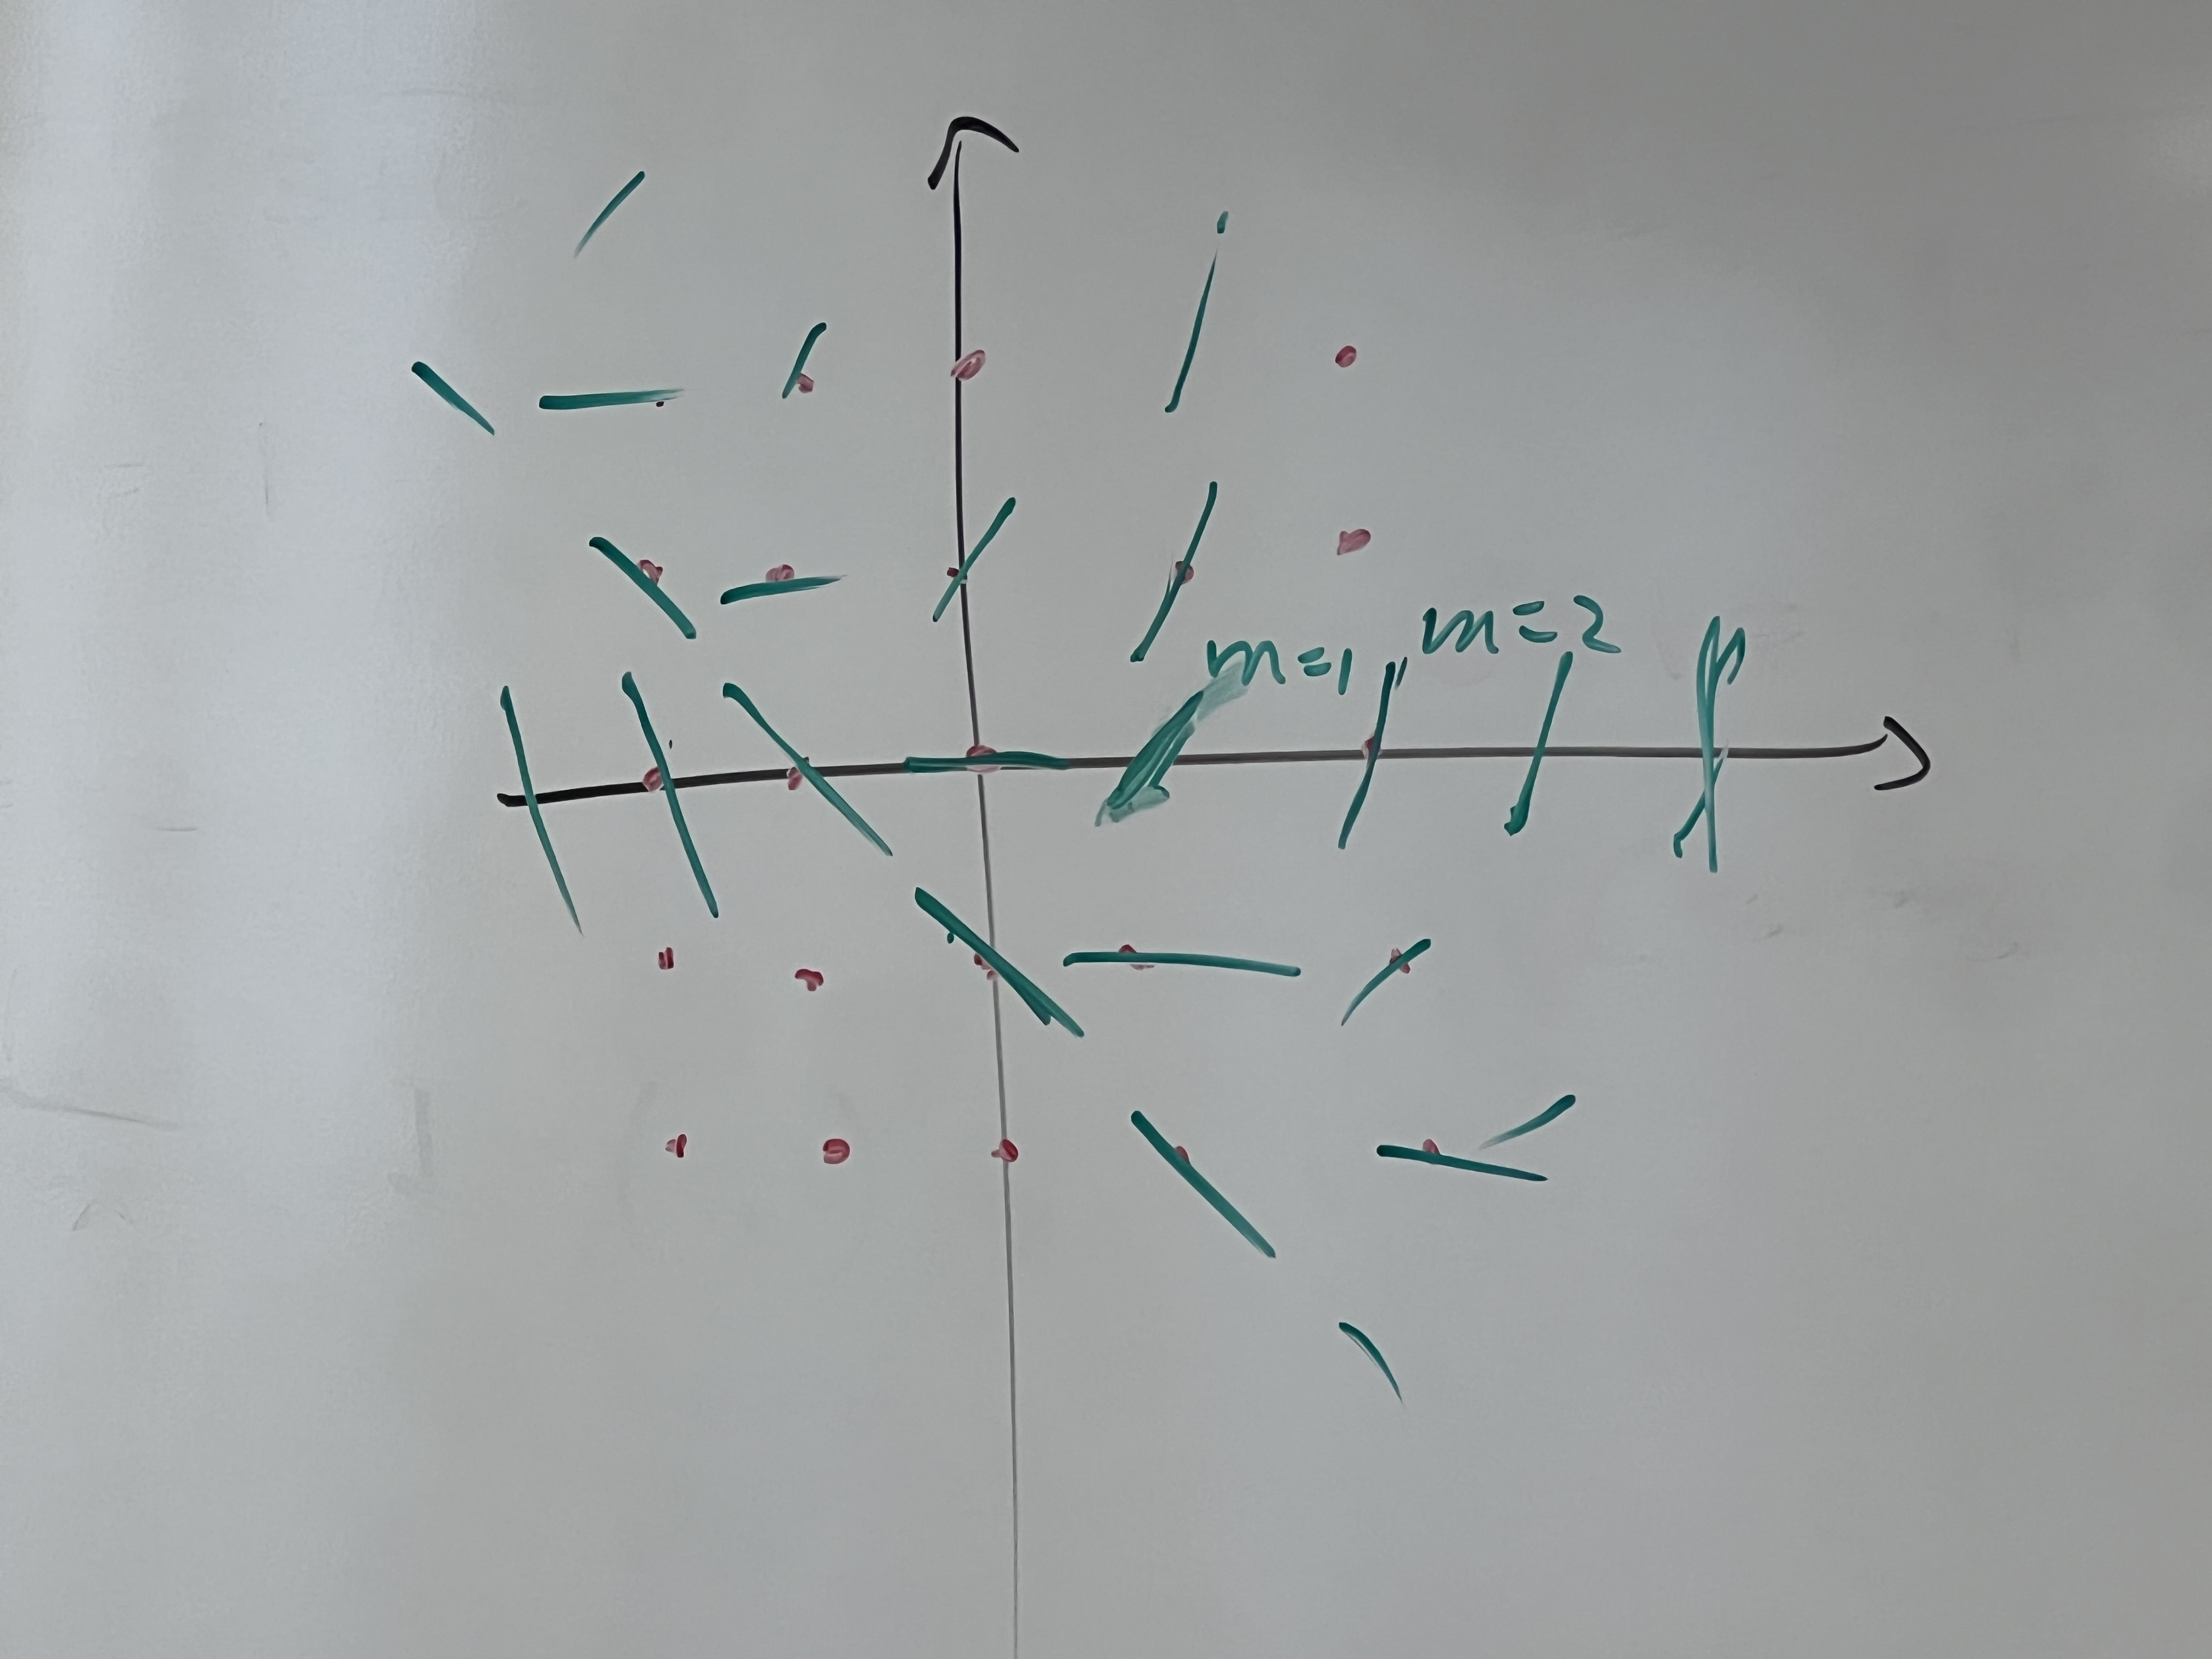
\includegraphics[width=\textwidth]{IMG_4767}
	\caption{The direction field for the previous example}
	\label{fig:direction-field-example}
\end{figure}

\noindent If the function $f(x,y)$ in the D.E. $y'=f(x,y)$ is reasonably simple so that we can solve $f(x,y)=0$, we can make a ``phase portrait diagram\label{dfn:phase-portrait-diagram}''. We will also assume $f(x,y)$ only involves the $y$-variable.

\example
\begin{equation*}
\begin{aligned}
	y'&=(y+2)(y-3)(y-5)\\
	f(x,y)&=(y+2)(y-3)(y-5)
\end{aligned}
\end{equation*}

An ``equilibrium solution\label{dfn:equilibrium-solution}'' is a solution where $y$ is a constant. In this example: $y=3$, $y=5$, $y=-2$ are each constant functions.

\begin{figure}[H]
	\centering
	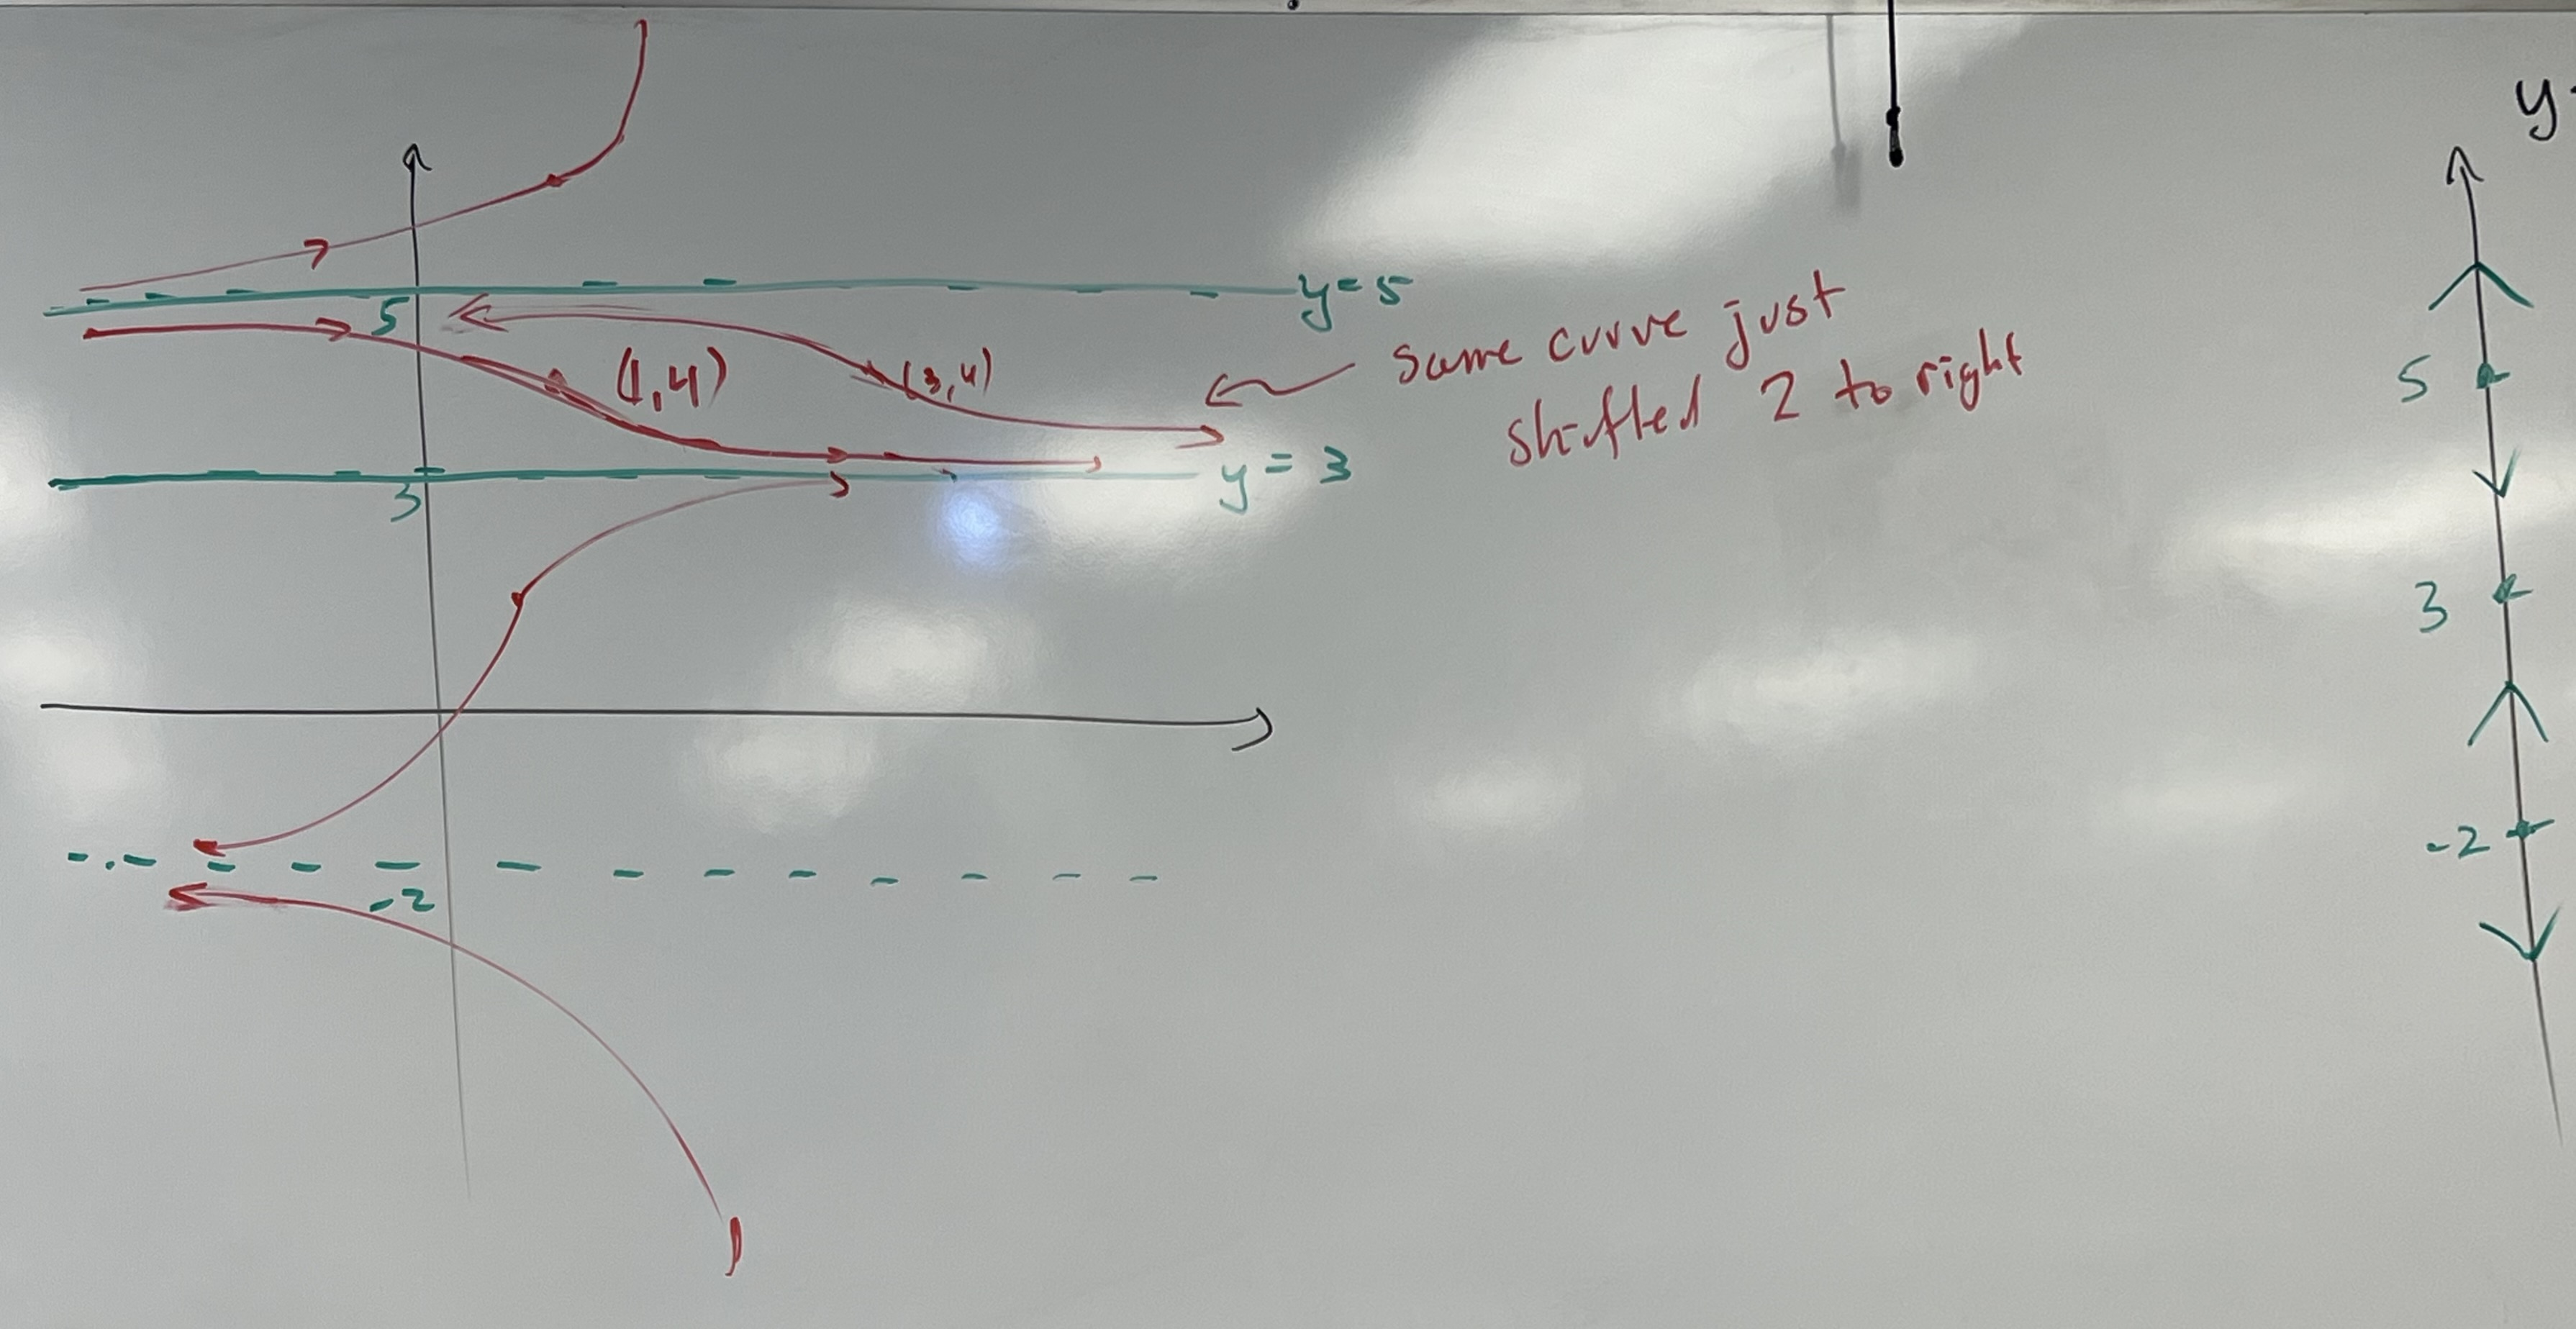
\includegraphics[width=\textwidth]{IMG_4770}
	\caption{The equilibrium solution for the previous example.}
	\label{fig:equilibrium-solution}
\end{figure}

\noindent The area around $y=5$ is an unstable equilibrium since the solutions diverge and go in separate directions away from $y=5$. The area around $y=3$ is a stable equilibrium because the slopes above and below it converge to $y=3$. The area around $y=-2$ is semi-stable, since all the slopes around it will converge in one direction, but the point isn't always $y=-2$.

%</Section-2.1>

\end{document}